\documentclass{ximera}
\title{Randomized Graphing}
% \subsubsection{Automatically load preambles and/or printstyles}
% \DescribeMacro{\xmDefaultPreamble}{ximeraPreamble.tex}
% \DescribeMacro{\xmDefaultPrinstyle}{ximeraPrintstyle.sty}
%   doc todo
%    \begin{macrocode}
%<*classXimera>
% If somewhere a file \xmDefaultPreamble (default:ximerapreamble.tex) 
% is found: load it
\def\input@path{{./}{../}{../../}{../../../}}    % Mmm, do we need to reset it to the previous value ?
\providecommand{\xmDefaultPreamble}{ximeraPreamble.tex}
    \IfFileExists{\xmDefaultPreamble}
    {
        \typeout{Loading Ximera defaultPreamble \xmDefaultPreamble}
        \input{\xmDefaultPreamble}
    }{
        \typeout{Info: No default preamble loaded (\xmDefaultPreamble)}
    }
\providecommand{\xmDefaultPrintstyle}{ximeraPrintstyle.sty}
\iftikzexport\else   % only in PDF        
    \IfFileExists{\xmDefaultPrintstyle}
    {
        \typeout{Loading Ximera defaultPrintstyle \xmDefaultPrintstyle}
        \input{\xmDefaultPrintstyle}
    }{
        \typeout{Info: No default printstyle loaded (\xmDefaultPrintstyle)}
    }    
\fi

%</classXimera>
%   \end{macrocode}



\begin{abstract}
    Attempts at randomizing graphing.
\end{abstract}
\begin{document}%

\maketitle




\subsection*{Ways to generate randomized graphs (Still being worked on)}

\subsubsection*{Using sageOutput environment}

\begin{sageOutput}
def RandInt(a,b):
    """ Returns a random integer in [`a`,`b`]. Note that `a` and `b` should be integers themselves to avoid unexpected behavior.
    """
    return QQ(randint(int(a),int(b)))
    # return choice(range(a,b+1))

def NonZeroInt(b,c, avoid = [0]):
    """ Returns a random integer in [`b`,`c`] which is not in `av`. 
        If `av` is not specified, defaults to a non-zero integer.
    """
    while True:
        a = RandInt(b,c)
        if a not in avoid:
            return a

p1temp1 = 'temp'

p1temp2 = x^2 + NonZeroInt(-2,2)
plot(p1temp2,(x,-3,3))
\end{sageOutput}

\begin{sagesilent}
def RandInt(a,b):
    """ Returns a random integer in [`a`,`b`]. Note that `a` and `b` should be integers themselves to avoid unexpected behavior.
    """
    return QQ(randint(int(a),int(b)))
    # return choice(range(a,b+1))

def NonZeroInt(b,c, avoid = [0]):
    """ Returns a random integer in [`b`,`c`] which is not in `av`. 
        If `av` is not specified, defaults to a non-zero integer.
    """
    while True:
        a = RandInt(b,c)
        if a not in avoid:
            return a

p1temp1 = 'temp'

p1temp2 = x^2 + NonZeroInt(-2,2)
plot(p1temp2,(x,-3,3))
\end{sagesilent}


Note that everything inside a sageOutput environment is essentially locked into it's own scope - no using variables from in there to populate environments elsewhere on the page (e.g. no using the same random number to define a function in a problem, and display a function on the page - that I've found).

Above is (probably) NOT a graph of $\sage{p1temp2}$ for example.

$\sageplot{plot(p1temp2, -1, 1)}$


$\sagestr{p1temp1}$


\sagestr{p1temp1}

\subsubsection*{Using Desmos}



Desmos graph command seems.... broken maybe?

Let's make sure tikz still works:

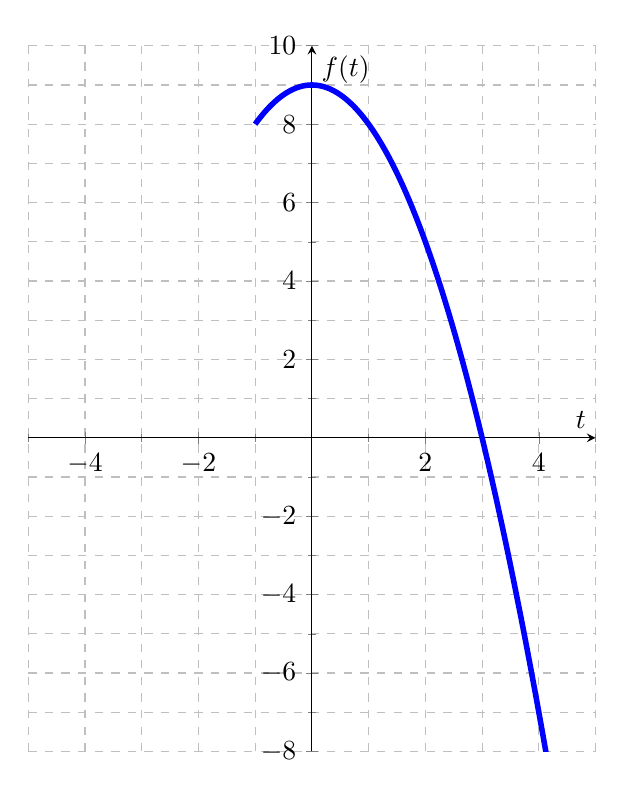
\begin{tikzpicture}
	\begin{axis}
		[
		width=250,
		height=300,
		xmin=-5, xmax=5,
		ymin=-8, ymax=10,
		grid=both,axis lines = middle, minor tick num = 1,
		grid style = dashed,
		xtick distance =2,ytick distance=2,
		xlabel = $t$, ylabel = $f(t)$
		]
		\addplot[domain = -1:10, line width = 2pt, color = blue,smooth,samples=200]{-1*(x)^2+9};
	\end{axis}
\end{tikzpicture}






\end{document}